%=======================================================================
% riscv-privileged.tex
%-----------------------------------------------------------------------

\documentclass[twoside,11pt]{book}
\setcounter{tocdepth}{4}
\setcounter{secnumdepth}{4}

% Package includes

\usepackage{graphicx}
\usepackage{geometry}
\usepackage{array}
\usepackage{colortbl}
\usepackage[colorlinks=true,linkcolor=blue]{hyperref}
\usepackage{placeins}
\usepackage{bbding}
\usepackage{longtable}
\usepackage{multirow}
\usepackage{float}

\usepackage{tabulary}
\usepackage{listings}
\usepackage{algorithmicx}
\usepackage{program}
\usepackage[nochapter]{vhistory}
% If LaTeX just doesn't do what I want, buy http://www.amazon.com/gp/product/0201362996

% Used for tables that can span pages:
\usepackage{xtab}

% Keep spacing normal in enumerated instead of adding extra space between
% items.
\usepackage{enumitem}
%\setlist{nolistsep}

\newenvironment{steps}[1]
  {
     \vspace{1ex}
     \noindent
     #1
     \begin{enumerate}
  }
  {
     \end{enumerate}
     \vspace{1ex}
 }

% Setup margins

\setlength{\topmargin}{-0.5in}
\setlength{\textheight}{9in}
\setlength{\oddsidemargin}{0in}
\setlength{\evensidemargin}{0in}
\setlength{\textwidth}{6.5in}

% Useful macros

\newcommand{\note}[1]{{\bf [ NOTE: #1 ]}}
\newcommand{\fixme}[1]{{\bf [ FIXME: #1 ]}}
\newcommand{\todo}[1]{\marginpar{\footnotesize #1}}

\newcommand{\wunits}[2]{\mbox{#1\,#2}}
\newcommand{\um}{\mbox{$\mu$m}}
\newcommand{\xum}[1]{\wunits{#1}{\um}}
\newcommand{\by}[2]{\mbox{#1$\times$#2}}
\newcommand{\byby}[3]{\mbox{#1$\times$#2$\times$#3}}

\newlength\savedwidth
\newcommand\whline[1]{%
  \noalign{%
    \global\savedwidth\arrayrulewidth\global\arrayrulewidth 1.5pt%
  }%
  \cline{#1}%
  \noalign{\vskip\arrayrulewidth}%
  \noalign{\global\arrayrulewidth\savedwidth}%
}

% Custom list environments

\newenvironment{tightlist}
{\begin{itemize}
 \setlength{\parsep}{0pt}
 \setlength{\itemsep}{-2pt}}
{\end{itemize}}

\newenvironment{titledtightlist}[1]
{\noindent
 ~~\textbf{#1}
 \begin{itemize}
 \setlength{\parsep}{0pt}
 \setlength{\itemsep}{-2pt}}
{\end{itemize}}

\newenvironment{commentary}
{ \vspace{-0.2in}
  \begin{quotation}
  \noindent
  \small \em
  \rule{\linewidth}{1pt}\\
}
{ 
  \end{quotation}
  \vspace{-0.2in}
}

% Other commands and parameters

\pagestyle{myheadings}
\setlength{\parindent}{0in}
\setlength{\parskip}{10pt}
\sloppy

% Commands for register format figures.

% New column types to use in tabular environment for instruction formats.
% Allocate 0.18in per bit.
\newcolumntype{I}{>{\centering\arraybackslash}p{0.18in}}
% Two-bit centered column.
\newcolumntype{W}{>{\centering\arraybackslash}p{0.36in}}
% Three-bit centered column.
\newcolumntype{F}{>{\centering\arraybackslash}p{0.54in}}
% Four-bit centered column.
\newcolumntype{Y}{>{\centering\arraybackslash}p{0.72in}}
% Five-bit centered column.
\newcolumntype{R}{>{\centering\arraybackslash}p{0.9in}}
% Six-bit centered column.
\newcolumntype{S}{>{\centering\arraybackslash}p{1.08in}}
% Seven-bit centered column.
\newcolumntype{O}{>{\centering\arraybackslash}p{1.26in}}
% Eight-bit centered column.
\newcolumntype{E}{>{\centering\arraybackslash}p{1.44in}}
% Ten-bit centered column.
\newcolumntype{T}{>{\centering\arraybackslash}p{1.8in}}
% Twelve-bit centered column.
\newcolumntype{M}{>{\centering\arraybackslash}p{2.2in}}
% Sixteen-bit centered column.
\newcolumntype{K}{>{\centering\arraybackslash}p{2.88in}}
% Twenty-bit centered column.
\newcolumntype{U}{>{\centering\arraybackslash}p{3.6in}}
% Twenty-bit centered column.
\newcolumntype{L}{>{\centering\arraybackslash}p{3.6in}}
% Twenty-five-bit centered column.
\newcolumntype{J}{>{\centering\arraybackslash}p{4.5in}}

\newcommand{\instbit}[1]{\mbox{\scriptsize #1}}
\newcommand{\instbitrange}[2]{~\instbit{#1} \hfill \instbit{#2}~}
\newcommand{\reglabel}[1]{\hfill {\tt #1}\hfill\ }

\newcommand{\wiri}{\textbf{WIRI}}
\newcommand{\wpri}{\textbf{WPRI}}
\newcommand{\wlrl}{\textbf{WLRL}}
\newcommand{\warl}{\textbf{WARL}}





% All registers are named here. That way when we rename one we'll get errors if
% there are still references to the old name.

\usepackage{makeidx}
\makeindex

\usepackage{xspace}
\newcommand{\defregname}[2]{\providecommand{#1}{{\tt #2}\xspace}}
\newcommand{\deffieldname}[2]{\providecommand{#1}{{$|#2|$}\xspace}}
\deffieldname{\Fmprv}{mprv}
\defregname{\Rmstatus}{mstatus}

\defregname{\Azero}{a0}
\defregname{\Aone}{a1}

\defregname{\Rzero}{zero}
\defregname{\Szero}{s0}
\defregname{\Sone}{s1}

\defregname{\Tzero}{t0}

\defregname{\Xzero}{x0}
\defregname{\Xone}{x1}
\defregname{\Xeight}{x8}
\defregname{\Xnine}{x9}
\defregname{\Xten}{x10}
\defregname{\Xeleven}{x11}
\defregname{\Xthirtyone}{x31}
\defregname{\Fone}{f1}
\defregname{\Rpc}{pc}
\defregname{\Rmhartid}{mhartid}
\defregname{\Rmepc}{mepc}

\input{hwbp_registers.tex.inc}
\input{core_registers.tex.inc}
\input{jtag_registers.tex.inc}
\input{dm_registers.tex.inc}
\input{sample_registers.tex.inc}
\input{abstract_commands.tex.inc}
<registers name="Virtual Core Debug Registers" prefix="VIRT_">
  Users of the debugger shouldn't need to know about the core debug registers,
  but may want to change things affected by them. 
     A virtual register is one that doesn't exist directly in the hardware, but that the debugger exposes as if it does. 
    
     <register name="Privilege Level" short="priv" address="virtual">
        User can read this register to  inspect the privilege level that
        the hart was running in when the hart halted.
        User can write this register to change the privilege level that
        the hart will run in when it resumes.

        \begin{table}
        \centering
        \caption{Privilege Level Encoding}
        \label{tab:privlevel}
        \begin{tabular}{|r|l|}
        \hline
        Encoding &amp; Privilege Level \\
        \hline
        0 &amp; User/Application \\
        1 &amp; Supervisor \\
        2 &amp; Hypervisor \\
        3 &amp; Machine \\
        \hline
        \end{tabular}
        \end{table}

        <field name="prv" bits="1:0" access="R/W" reset="0">
            Contains the privilege level the hart was operating in when Debug
            Mode was entered. The encoding is described in Table
            \ref{tab:privlevel}. A user can write this value to change the
            hart's privilege level when exiting Debug Mode.
        </field>
    </register>
</registers>

<registers name="Debug Module Debug Bus Registers" prefix="DMI_">

    <!-- =============== serial ports =============== -->

    <register name="Serial Control and Status" short="sercs" address="0x34">
        If \Fserialcount is 0, this register is not present.

        <field name="serialcount" bits="31:28" access="R" reset="Preset">
            Number of supported serial ports.
        </field>
        <field name="0" bits="27" access="R" reset="0" />
        <field name="serial" bits="26:24" access="R/W" reset="0">
            Select which serial port is accessed by \Rserrx and \Rsertx.
        </field>
        <field name="error7" bits="23" access="R/W1C" reset="0"/>
        <field name="valid7" bits="22" access="R" reset="0" />
        <field name="full7" bits="21" access="R" reset="0" />
        <field name="error6" bits="20" access="R/W1C" reset="0"/>
        <field name="valid6" bits="19" access="R" reset="0" />
        <field name="full6" bits="18" access="R" reset="0" />
        <field name="error5" bits="17" access="R/W1C" reset="0"/>
        <field name="valid5" bits="16" access="R" reset="0" />
        <field name="full5" bits="15" access="R" reset="0" />
        <field name="error4" bits="14" access="R/W1C" reset="0"/>
        <field name="valid4" bits="13" access="R" reset="0" />
        <field name="full4" bits="12" access="R" reset="0" />
        <field name="error3" bits="11" access="R/W1C" reset="0"/>
        <field name="valid3" bits="10" access="R" reset="0" />
        <field name="full3" bits="9" access="R" reset="0" />
        <field name="error2" bits="8" access="R/W1C" reset="0"/>
        <field name="valid2" bits="7" access="R" reset="0" />
        <field name="full2" bits="6" access="R" reset="0" />
        <field name="error1" bits="5" access="R/W1C" reset="0"/>
        <field name="valid1" bits="4" access="R" reset="0" />
        <field name="full1" bits="3" access="R" reset="0" />
        <field name="error0" bits="2" access="R/W1C" reset="0">
            1 when the debugger-to-core queue for serial port 0 has
            over or underflowed. This bit will remain set until it is reset by
            writing 1 to this bit.
        </field>
        <field name="valid0" bits="1" access="R" reset="0">
            1 when the core-to-debugger queue for serial port 0 is not empty.
        </field>
        <field name="full0" bits="0" access="R" reset="0">
            1 when the debugger-to-core queue for serial port 0 is full.
        </field>
    </register>

    <register name="Serial TX Data" short="sertx" address="0x35">
        If \Fserialcount is 0, this register is not present.

        This register provides access to the write data queue of the serial port
        selected by \Fserial in \Rsercs.

        If the {\tt error} bit is not set and the queue is not full, a write to this register
        adds the written data to the core-to-debugger queue.
        Otherwise the {\tt error} bit is set and the write returns error.

        A read to this register returns the last data written.

        <field name="data" bits="31:0" access="R/W" reset="0" />
    </register>

    <register name="Serial RX Data" short="serrx" address="0x36">
        If \Fserialcount is 0, this register is not present.

        This register provides access to the read data queues of the serial port
        selected by \Fserial in \Rsercs.

        If the {\tt error} bit is not set and the queue is not empty, a read from this register reads the
        oldest entry in the debugger-to-core queue, and removes that entry from the queue.
        Otherwise the {\tt error} bit is set and the read returns error.

        <field name="data" bits="31:0" access="R" reset="0" />
    </register>
</registers>


\input{vc.tex}

\newcommand{\versionnum}{0.13}


\begin{document}

\title{RISC-V External Debug Support\\
Version \versionnum\\
\GITHash
}
\author{Tim Newsome \textless tim@sifive.com\textgreater}
\date{\GITAuthorDate}
\maketitle

\markboth{RISC-V External Debug Support Version \versionnum}
{RISC-V External Debug Support Version \versionnum}
\thispagestyle{empty}

\frontmatter

\chapter{Preface}

{\bf Warning! This draft specification will change before being accepted as
standard, so implementations made to this draft specification will likely not
conform to the future standard.}


\section*{Acknowledgments}

I would like to thank the following people for their time, feedback, and ideas:
Bruce Ableidinger,
Krste Asanovic,
Mark Beal,
Alex Bradbury,
Zhong-Ho Chen,
Monte Dalrymple,
Vyacheslav Dyanchenco,
Peter Egold,
Richard Herveille,
Po-wei Huang,
Scott Johnson,
Aram Nahidipour,
Rishiyur Nikhil,
Gajinder Panesar,
Klaus Kruse Pedersen,
Antony Pavlov,
Ken Pettit,
Wesley Terpstra,
Megan Wachs,
Stefan Wallentowitz,
Ray Van De Walker,
Andrew Waterman,
and Andy Wright.


\tableofcontents
\listoffigures
\listoftables

\mainmatter

\newpage

\chapter{Introduction}
\label{sec:intro}

When a design progresses from simulation to hardware implementation, a user's
control and understanding of the system's current state drops dramatically.
To help bring up and debug low level software and hardware,
it is critical to have good debugging support built into the hardware.
When a robust OS is running on a core, software can handle many
debugging tasks. However, in many scenarios, hardware support is essential.

This document outlines a standard architecture for external debug support 
on RISC-V platforms. This architecture allows a variety of implementations and
tradeoffs, which is complementary to the wide range of RISC-V implementations.
At the same time, this specification defines common interfaces to
allow debugging tools and components to target a variety of platforms based on the RISC-V ISA.

System designers may choose to add additional hardware debug support,
but this specification defines a standard interface for common
functionality.

\section{Terminology}

A \emph{platform} is a single integrated circuit consisting of one or more
\emph{components}. Some components may be RISC-V cores, while others may have a different
function. Typically they will all be connected to a single system bus.
A single RISC-V core contains one or more hardware threads, called
\emph{harts}.

\section{About This Document}

\subsection{Structure}

This document contains two parts. The main part of the document is the
specification, which is given in the numbered sections. The second part
of the document is a set of  appendices. The information
in the appendix is intended to clarify and provide examples, but is
not part of the actual specification.


\subsection{Register Definition Format}

All register definitions in this document follow the format shown in Section~\ref{shortname}.
A simple graphic shows which fields are in the register. The
upper and lower bit indices are shown to the top left and top right of each
field. The total number of bits in the field are shown below it.

After the graphic follows a table which for each field lists its name,
description, allowed accesses, and reset value. The allowed accesses are listed
in Table~\ref{tab:access}.

\begin{table}[htp]
    \centering
    \caption{Register Access Abbreviations}
    \label{tab:access}
    \begin{tabulary}{\textwidth}{|l|L|}
        \hline
        R & Read-only. \\
        \hline
        R/W & Read/Write. \\
        \hline
        R/W0 & Read/Write. Only writing 0 has an effect.  \\
        \hline
        R/W1 & Read/Write. Only writing 1 has an effect.  \\
        \hline
        R/W1C & Read/Write. For each bit in the field, writing 1 clears that bit. Writing 0 has no effect. \\
        \hline
        W & Write-only. When read this field returns 0. \\
        \hline
        W1 & Write-only. Only writing 1 has an effect. \\
        \hline
    \end{tabulary}
\end{table}

\input{sample_registers.tex}

%\section{Reading Order}

This section describes the minimal parts of the spec required to understand a
given piece of functionality. It's still best to read the whole thing, but it
might help you get started better than reading it all start to finish. No
matter what you want to learn about, it's best to read Section~\ref{overview}
first.

\subsubsection{Halt/Resume}

Sections \ref{dmi}, \ref{selectingharts}, \ref{haltcontrol}, \ref{dmcontrol}, \ref{dmstatus},
\ref{haltsum}, \ref{deb:halt}.

\subsubsection{Abstract Register Access}

Sections \ref{abstractcommands}, \ref{abstractcs}, \ref{command},
\ref{data0}, \ref{deb:abstractreg}.

\subsubsection{Program Buffer}

Sections \ref{programbuffer}, \ref{progbufcs}, \ref{progbuf0}, \ref{access
register}, \ref{debugmode}, \ref{deb:regprogbuf}, \ref{deb:mrprogbuf}.

\subsubsection{JTAG Debug Transport Module}

Sections \ref{dtm}, \ref{jtagdtm}, \ref{dbusaccess}.

\subsubsection{System Bus Master}

Sections \ref{systembusaccess}, \ref{sbcs}, \ref{sbaddress0}, \ref{sbaddress1},
\ref{sbaddress2}, \ref{sbdata0}, \ref{sbdata1}, \ref{sbdata2}, \ref{sbdata3},
\ref{deb:mrsysbus}.

\subsubsection{Reset}

TODO

\subsubsection{Security}

TODO

\subsubsection{Triggers}

TODO

\subsubsection{Serial Ports}

TODO



\section{Background}

There are several use cases for dedicated debugging hardware, both
internal to a CPU core and with an external connection.
This specification addresses the the use cases listed below. Implementations
can choose to not to implement every feature, which means some use cases might
not be supported.

\begin{itemize}

\item Debugging low-level software in the absence of an OS or other software.

\item Debugging issues in the OS itself.

\item Bootstrapping a system to test, configure, and program components before
  there is any executable code path in the system.

\item Accessing hardware on a system without a working CPU.

\end{itemize}

In addition, even without a hardware debugging interface,
architectural support in a RISC-V CPU can aid software debugging and
performance analysis by allowing hardware triggers and breakpoints.
This specification aims to define common resources which can be used
for different cases.

When debugging software, this specification distinguishes between two
forms of external debugging. The first is \emph{halt mode} debugging,
where an external debugger halts some or all components of a
platform and inspects their state while they are in stasis.
The debugger can read and/or modify state, then direct the hardware
to execute a single instruction, or continue to run freely.

The second is \emph{run mode} debugging. In this mode a software
debug agent runs on a component (eg.  triggered by a timer interrupt or breakpoint
on a RISC-V core) which transfers data to or from the debugger
without halting the component, only briefly interrupting its program flow.
This functionality is essential if the component is controlling some real-time system (like a
hard drive) where long timing delays could lead to physical damage.
This requires additional software support (both on the system as well as on the debugger),
and efficient communication channels between the component and the debugger.

%MAW -- where does Quick Access fit in the above description? Is it fair to call
% it run-mode debugging?

\section{Supported Features}

The debug interface described in this specification supports the following features:

\begin{enumerate}
   \item RV32, RV64, and future RV128 are all supported.
   \item Any hart in the platform can be independently debugged.
   \item A debugger can discover almost everything it needs to know itself,
       without user configuration.
   \item Each hart can be debugged from the very first instruction executed.
   \item A RISC-V hart can be halted when a software breakpoint instruction is
       executed.
   \item Hardware single-step can execute one instruction at a time.
   \item Debug functionality is independent of the debug transport used.
   \item The debugger does not need to know anything about the microarchitecture
       of the cores it is debugging.

   \item Arbitrary subsets of harts can be halted and resumed simultaneously.
       (Optional)
   \item Arbitrary instructions can be executed on
       a halted hart. That means no new debug functionality is needed when a
       core has additional or custom instructions or state, as
       long as there exist programs
       that can move that state into GPRs. (Optional)
   \item Registers can be accessed without halting. (Optional)
   \item A running hart can be directed to execute a short sequence
       of instructions, with little overhead. (Optional)
   \item A system bus master allows memory access without
       involving any hart. (Optional)
   \item A RISC-V hart can be halted when a trigger matches the PC,
       read/write address/data, or an instruction opcode. (Optional)
\end{enumerate}

This document does not suggest a strategy or implementation for hardware test,
debugging or error detection techniqes. Scan, BIST, etc. are out of scope of
this specification, but this specification does not intend to limit their use 
in RISC-V systems.

\chapter{System Overview} \label{overview}

Figure~\ref{fig:overview} shows the main components of External Debug Support.
Blocks shown in dotted lines are optional. 

\begin{figure}
   \centering
   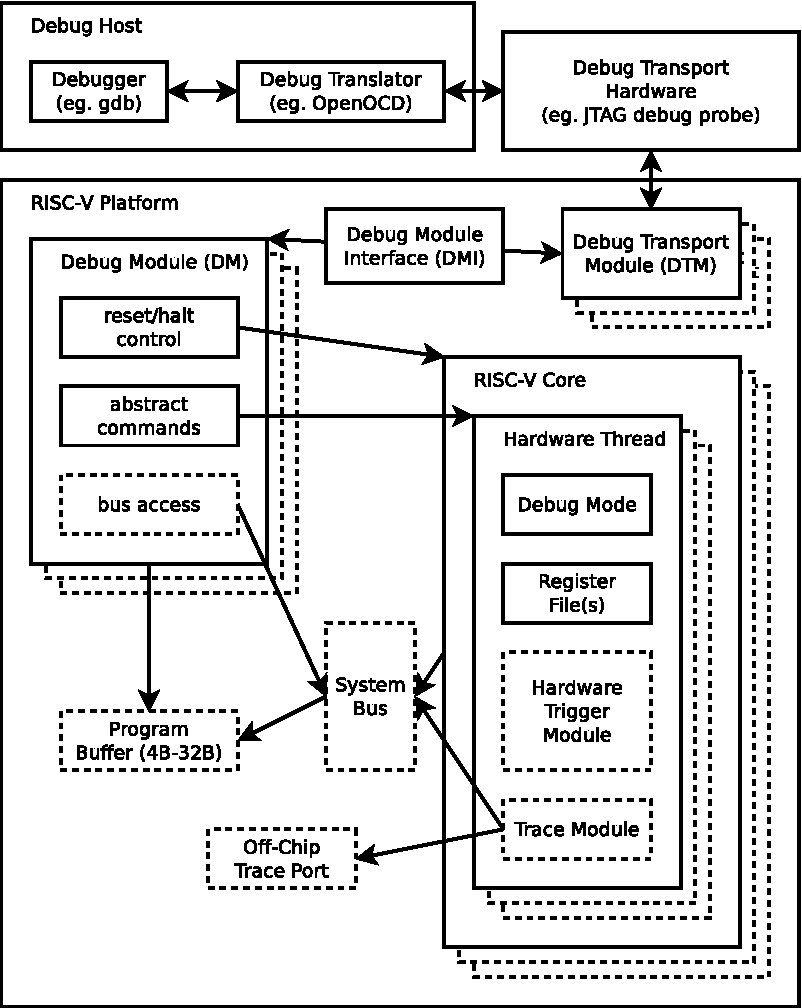
\includegraphics[width=\textwidth]{fig/overview-eps-converted-to.pdf}
   \caption{RISC-V Debug System Overview}
   \label{fig:overview}
\end{figure}

The user interacts with the Debug Host (eg. laptop), which is running a
debugger (eg. gdb).  The debugger communicates with a Debug Translator (eg.
OpenOCD, which may include a hardware driver) to communicate with Debug
Transport Hardware (eg.  Olimex USB-JTAG adapter).
The Debug Transport Hardware connects the Debug Host to the Platform's Debug
Transport Module (DTM).  The DTM provides access to the Debug Module (DM) using
the Debug Module Interface (DMI).

The DM allows the debugger to halt any hart in the platform. Abstract commands
provide access to GPRs.
The optional Program Buffer allows the debugger to execute arbitrary code on the hart,
which allows access to additional hart state. Alternatively, additional
abstract commands can provide access to additional hart state.

Each RISC-V hart may implement a Trigger Module. When trigger conditions
are met, harts will halt and inform the debug module that they have
halted.

An optional system bus access block allows memory accesses without using a
RISC-V hart to perform the access.

Optional serial port blocks may allow the Debug Transport to be re-used as a
generic communication interface. This functionality is out of the
scope of this specification.


\chapter{Debug Module (DM)} \label{dm}

\begin{steps}{The Debug Module implements a translation interface between abstract debug
    operations and their specific implementation. It might support the following
    operations:}
\item Give the debugger necessary information about the implementation. (Required)
\item Allow any individual hart to be halted and resumed. (Required)
\item Provide status on which harts are halted. (Required)
\item Provide read and write access to a halted hart's GPRs. (Required)
\item Provide access to a reset signal that allows debugging from the very
    first instruction after reset. (Required)
\item Provide access to other hart registers. (Optional)
\item Provide a Program Buffer to force the hart to execute arbitrary instructions. (Optional)
\item Allow multiple harts to be halted, resumed, and/or reset at the same time. (Optional)
\item Allow direct System Bus Access. (Optional)
\end{steps}

In order to implement memory access, a target must implement either the Program
Buffer or System Bus Access.

A single DM can debug up to 1024 harts.

\section{Debug Module Interface (DMI)} \label{dmi}

The Debug Module is a slave to a bus called the Debug Module Interface (DMI). The
master of the bus is the Debug Transport Module(s).
The Debug Module Interface can be a trivial bus with one master and one slave,
or use a more full-featured bus like TileLink or the AMBA Advanced Peripheral
Bus. The details are left to the system designer.

The DMI uses between 7 and 32 address bits.  It supports read and write
operations.  The bottom of the address space is
used for the DM. Extra space can be used for custom debug devices, other cores,
additional DMs, etc.

The Debug Module is controlled via register accesses to its DMI address space.

\begin{table}[htp]
    \centering
    \caption{Debug Module Interface Address Space}
    \label{tab:header}
    \begin{tabulary}{\textwidth}{|r|L|}
        \hline
        0x00 -- 0x3f & Registers described in Section~\ref{dmdebbus}. \\
        \hline
        0x40 -- 0x5f & This is called the `halt region`.  These 32 addresses
        for 32-bit words provide access to the halt bit for up to 1024 harts.
        If the hart is halted, the bit is 1.  Otherwise
        the bit is 0. The bit for hart 0 is the LSB in the 32-bit word at 0x40.
        The bit for hart 1023 is the MSB in the 32-bit word at 0x5f. \\
        \hline
    \end{tabulary}
\end{table}

\section{Reset Control} \label{reset}

The Debug Module controls a global reset signal, \Fndmreset (non-debug module
reset),
which can reset, or hold in reset, every component in the platform,
except for the Debug Module and Debug
Transport Modules.
Exactly what is affected by this reset is implementation dependent, as long as
it is possible to debug programs from the first instruction executed.
The Debug Module's own state and registers should only be
reset at power-up and while
\Fdmactive in \Rdmcontrol is 0.
The halt state of harts should be
maintained across system reset provided that \Fdmactive is 1,
although trigger CSRs may be cleared.

Due to clock and power domain crossing issues,
it may not be possible to perform arbitrary DMI accesses across
system reset.
While \Fndmreset or any external reset is asserted, the only supported DM
operation is accessing \Rdmcontrol. The behavior of other accesses is
undefined.

\section{Selecting Harts} \label{selectingharts}

Up to 1024 harts can be connected to a single DM. The debugger
selects a hart, and then subsequent halt, resume, reset, and debugging
commands are specific to that hart.

A debugger can enumerate all the harts
attached to the DM by selecting each hart starting from 0
until \Fanynonexistent in \Rdmstatus is 1.

The debugger can discover the mapping between hart indices and
\Rmhartid by using the interface to read \Rmhartid, or by
reading the system's Device Tree.

\subsection {Selecting a Single Hart}

All debug modules must support selecting a single hart.
The debugger can select a hart by writing its index to \Fhartsel.
Hart indexes start at 0 and are contiguous until the final index.

\subsection {Selecting Multiple Harts}

Debug Modules may optionally implement a Hart Array Mask register to allow
selecting multiple harts at once. The debugger can set bits in the hart array mask register
using \Rhawindowsel and \Rhawindow, then apply actions to all selected harts
by setting \Fhasel. If this feature is supported, multiple harts can be
halted, resumed, and reset simultaneously.

Only the actions initiated by \Rdmcontrol can apply to multiple harts
at once, Abstract Commands apply only to the hart selected by
\Fhartsel.

\section{Run Control} \label{runcontrol}

The Debug Module can halt selected harts and allow them to run again using
the \Rdmcontrol register.
After selecting harts, it sets \Fhaltreq, then waits for \Fallhalted to
indicate the harts are halted before clearing \Fhaltreq to 0. Setting \Fhaltreq
has no effect on harts which are already halted.

To resume, the debugger sets \Fresumereq. This action sets each selected hart's
{\tt resumeack} bit to 0. Once a hart has resumed, it
sets its {\tt resumeack} bit to 1. Thus, the
debugger should wait for \Fallresumeack to indicate all
harts have resumed before clearing \Fresumereq to 0.
If a debugger reads \Fanyresumeack and \Fanyhalted in the same operation, then
some selected harts must have resumed and then halted again.

\begin{commentary}
  When waiting for a hart to resume, a debugger should
  examine \Fallresumeack, not \Fallrunning
  or \Fallhalted,
  because the hart may immediately halt again due to
  trigger or step conditions.
\end{commentary}

Setting \Fresumereq on hart which is running
clears {\tt resumeack} but
may cause a hart which halts in the future to immediately
resume. Debuggers should not depend on this behavior and should not
set \Fresumereq for running harts.

To halt or resume multiple harts at the same time, the debugger first
sets the hart's bits in the hart array mask register, then
follows the same procedure but with \Fhasel set to 1.
Depending on the desired operation, the debugger might consider the {\tt any*}
versions of the status instead of {\tt all*}.

When halt or resume is requested, a hart must respond in
less than one second, unless it is unavailable.
(How this is implemented is not further specified. A few
clock cycles will be a more typical latency).

\section{Abstract Commands} \label{abstractcommands}

The DM supports a set of abstract commands, most of which
are optional. Depending on the implementation, the debugger may
be able to perform
some abstract commands even when the selected hart is not halted.
Debuggers can only determine which abstract commands
are supported by a given hart in a given state by attempting them
and then looking at \Fcmderr in \Rabstractcs to see if they were successful.

Debuggers execute abstract commands by writing them to \Rcommand.
Debuggers can determine whether an abstract command is complete by
reading \Fbusy in \Rabstractcs.
If the command takes arguments, the debugger
must write them to the {\tt data} registers before writing to \Rcommand. If a
command returns results, the Debug Module must ensure they are placed
in the {\tt data} registers before \Fbusy is cleared.
Which {\tt data} registers are used for the arguments is
described in Table~\ref{tab:datareg}.  In all cases the least-significant word
is placed in the lowest-numbered {\tt data} register.

\begin{table}[htp]
    \centering
    \caption{Use of Data Registers}
    \label{tab:datareg}
    \begin{tabulary}{\textwidth}{|r|l|l|l|}
        \hline
        XLEN & arg0/return value & arg1 & arg2 \\
        \hline
        32 & \Rdatazero & {\tt data1} & {\tt data2} \\
        \hline
        64 & \Rdatazero, {\tt data1}  & {\tt data2} , {\tt data3} & {\tt data4}, {\tt data5} \\
        \hline
        128 & \Rdatazero-- {\tt data3} & {\tt data4} -- {\tt data7} & {\tt data8} -- {\tt data11} \\
        \hline
    \end{tabulary}
\end{table}

\subsection{Abstract Command Listing}

This section describes each of the different abstract commands
and how their fields should be interpreted when
they are written to \Rcommand.

Each abstract command is a 32-bit value. The top 8 bits contain \Fcmdtype which
determines the kind of command. Table~\ref{tab:cmdtype} lists all commands.

\begin{table}[htp]
    \centering
    \caption{Meaning of \Fcmdtype}
    \label{tab:cmdtype}
    \begin{tabulary}{\textwidth}{|r|l|l|l|}
        \hline
        \Fcmdtype & Command & Page \\
        \hline
        0 & Access Register Command & \pageref{access register} \\
        \hline
        1 & Quick Access & \pageref{quick access} \\
        \hline
    \end{tabulary}
\end{table}

\input{abstract_commands.tex}

\begin{table}[htp]
    \centering
    \caption{Abstract Register Numbers}
    \label{tab:regno}
    \begin{tabulary}{\textwidth}{|r|l|}
        \hline
        0x0000 -- 0x0fff & CSRs. The ``PC'' can be accessed here through \Rdpc.
        \\
        \hline
        0x1000 -- 0x101f & GPRs \\
        \hline
        0x1020 -- 0x103f & Floating point registers \\
        \hline
        0xc000 -- 0xffff & Reserved for non-standard extensions and internal
        use. \\
        \hline
    \end{tabulary}
\end{table}

\section{Program Buffer} \label{programbuffer}

To support executing arbitrary instructions on a halted hart,
a Debug Module can include a Program Buffer that a debugger
can write small programs to. Systems
that support all necessary functionality using abstract commands
only may choose to omit the Program Buffer.

A debugger can write a small program to the Program Buffer, and then
execute it exactly once with the Access Register Abstract Command,
setting the \Fpostexec bit in \Rcommand.
The debugger can write whatever program it likes (including jumps out of the
Program Buffer), but the program must end with
{\tt ebreak} or {\tt ebreak.c}. To save hardware, an implementation may support
an implied {\tt ebreak} that is executed when a hart runs off the end of the
Program Buffer. With this feature, a Program Buffer of just 2 32-bit words can
offer efficient debugging.

If \Fprogbufsize is 1, the Program Buffer may only hold a single instruction,
and \Fimpebreak must be 1.
This instruction can be a 32-bit
instruction, or a compressed instruction in the lower 16 bits accompanied by a
compressed {\tt nop} in the upper 16 bits.

If the debugger executes a program that does not
terminate with an {\tt ebreak} instruction, the hart will remain in Debug Mode
until it is reset.

While these programs are executed, the hart does not leave Debug Mode (see
Section~\ref{debugmode}).  If an exception is encountered during execution of
the Program Buffer, no more instructions are executed, the hart remains in Debug
Mode, and \Fcmderr is set to 3 ({\tt exception error}).  If the debugger
executes a program that doesn't terminate, then it loses control of the hart.

Executing the Program Buffer may clobber \Rdpc. If that is the case, it must be
possible to read/write \Rdpc using an abstract command with \Fpostexec not set.
The debugger must attempt to save \Rdpc between halting and
executing a Program Buffer, and then restore \Rdpc before leaving Debug Mode.

\begin{commentary}
    Allowing Program Buffer execution to clobber \Rdpc allows for direct
    implementations that don't have a separate PC register, and do need to use
    the PC when executing the Program Buffer.
\end{commentary}

The Program Buffer may be implemented as RAM which is accessible to the
hart as RAM memory. A debugger can determine if this is the case by executing small
programs that attempt to write and read back relative to \Rpc while executing
from the Program Buffer.
If so, the debugger has more flexibility in what it can do with the program buffer.

\section{Overview of States}

Figure~\ref{fig:abstract_sm} shows a conceptual view of the states
passed through by a hart during run/halt debugging as influenced
by the different fields of \Rdmcontrol, \Rabstractcs, \Rabstractauto, and
\Rcommand.

\begin{figure}
   \centering
   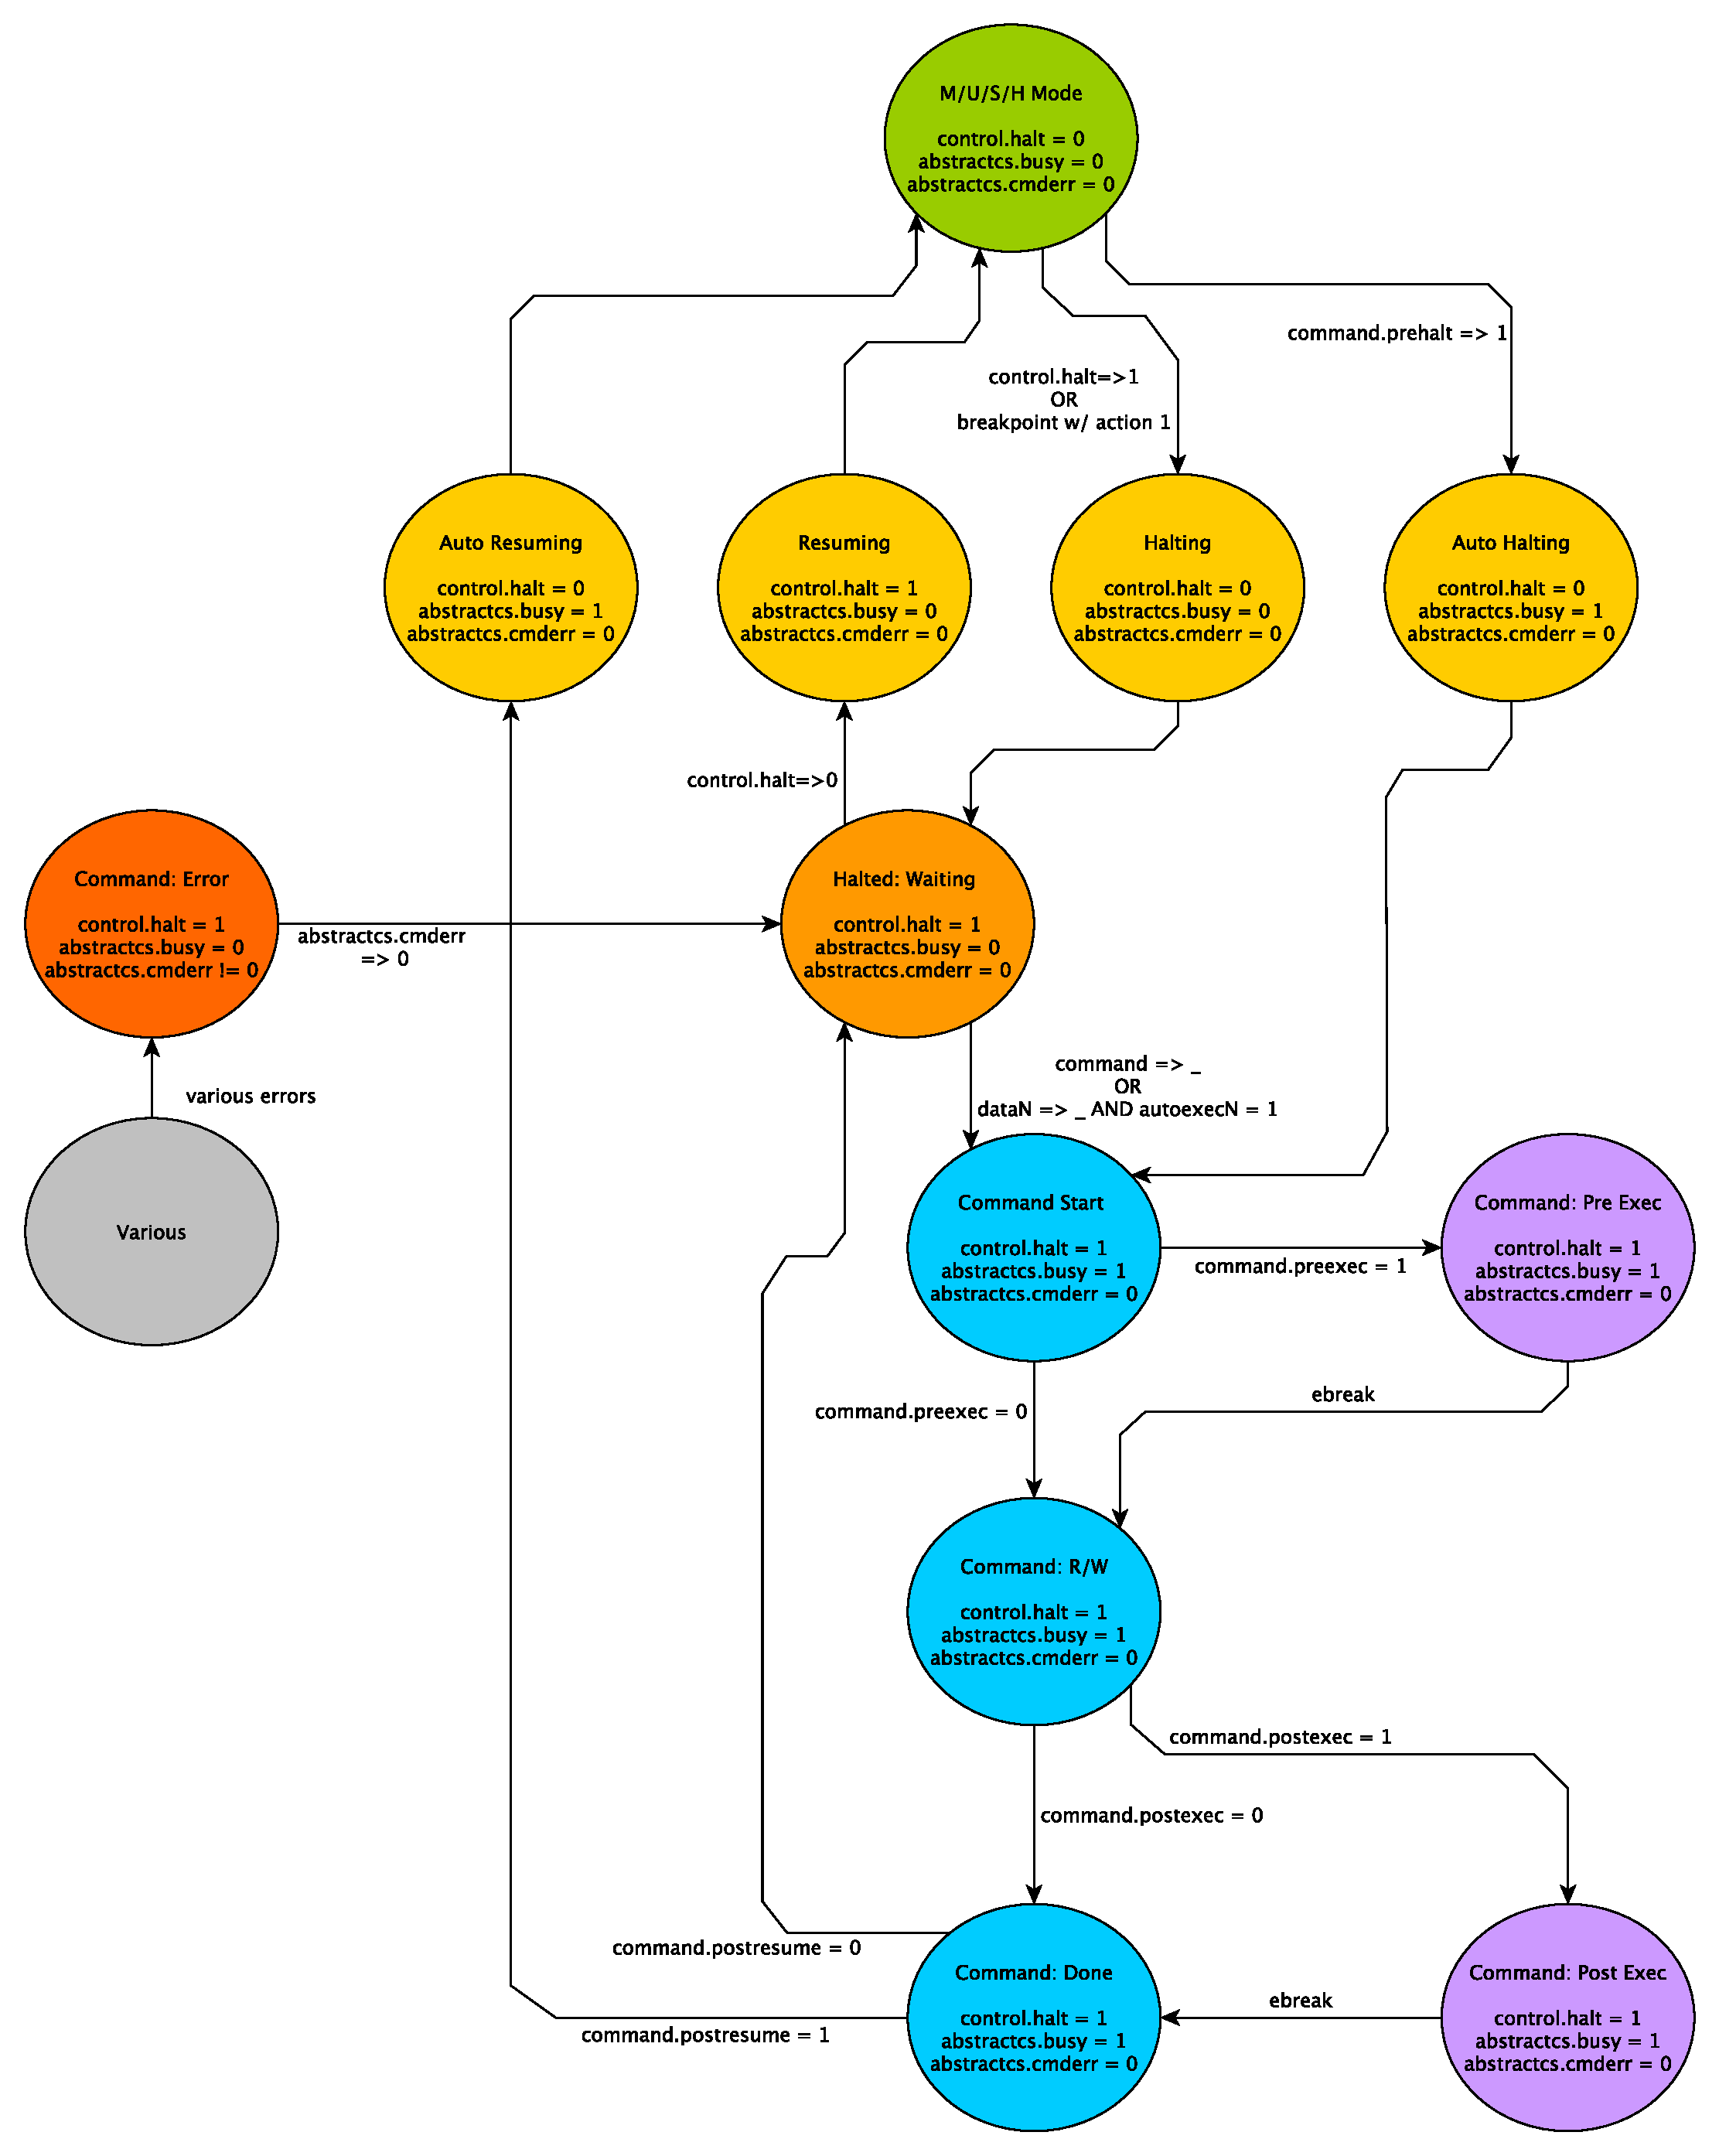
\includegraphics[width=\textwidth]{fig/abstract_commands.pdf}
   \caption[Run/Halt Debug State Machine]{Run/Halt Debug State Machine.
     As only a small amount of state is visibile to the debugger,
     the states and transitions are conceptual.}
   \label{fig:abstract_sm}
\end{figure}

\section{System Bus Access} \label{systembusaccess}

When a Program Buffer is present, a debugger can access the system bus by having a
RISC-V hart perform the accesses it requires.
A Debug Module may also include a System Bus Access block to provide memory
access without
involving a hart, regardless of whether Program Buffer is implemented.
The System Bus Access block uses physical addresses.

\begin{commentary}
Implementing a System Bus Access block has several benefits even
when a Debug Module also implements a Program Buffer. 
First, it is possible to
access memory in a running system with minimal impact.  Second, it may improve
performance when accessing memory.
Third, it may provide
access to devices that a hart does not have access to.
\end{commentary}

\section{Quick Access}

Depending on the task it is performing, some harts can only be halted very briefly.
There are several mechanisms that allow accessing resources in such a running system
with a minimal impact on the running hart.

First, an implementation may allow some abstract commands to execute without halting the hart.

Second, the Quick Access abstract command can be used to halt a hart, quickly
execute the contents of the Program Buffer, and let the hart run again.
Combined with instructions that allow Program Buffer code to access the
{\tt data} registers, as described in \ref{hartinfo}, this can be used to quickly
perform a memory or register access. For some systems this will be too
intrusive, but many systems that can't be halted can bear an occasional hiccup
of a hundred or less cycles.

Third, if the System Bus Access block is implemented, it can be used while a
hart is running to access system memory.

\section{Security}

To protect intellectual property it may be desirable to lock access to the
Debug Module.  To allow access during a manufacturing process and not
afterwards, a reasonable solution could be to add a fuse bit to the Debug
Module that can be used to be permanently disable it. Since this is technology
specific, it is not further addressed in this spec.

Another option is to allow the DM to be unlocked only by users who have an
access key. A few bits in \Rdmstatus and \Rauthdata can support an arbitrarily
complex authentication mechanism.  When \Fauthenticated is clear, the DM must
not interact with the rest of the platform in any way.

\section{Debug Module DMI Registers} \label{dmdebbus}

When read, unimplemented Debug Module DMI Registers return 0. Writing them has
no effect.

\input{dm_registers.tex}

\chapter{RISC-V Debug}
\label{sec:core_debug}

Modifications to the RISC-V core to support debug are kept to a minimum.  There
is a special execution mode (Debug Mode) and a few extra CSRs. The DM takes care
of the rest.

\section{Debug Mode} \label{debugmode}

Debug Mode is a special processor mode used only when the core is halted for
external debugging. How Debug Mode is implemented is not specified here.

\begin{steps}{When executing code from the Program Buffer, the processor stays
    in Debug Mode and the following apply:}
\item All operations are executed at machine mode privilege level, except that
    \Fmprv in \Rmstatus is ignored.
\item All interrupts are masked.
\item Exceptions don't update any registers.  That includes {\tt cause}, {\tt
    epc}, {\tt tval}, {\tt dpc}, and \Rmstatus. They do end execution of the
    Program Buffer.
\item No action is taken if a trigger matches.
\item Trace is disabled.
\item Counters may be stopped, depending on \Fstopcount in \Rdcsr.
\item Timers may be stopped, depending on \Fstoptime in \Rdcsr.
\item The {\tt wfi} instruction acts as a {\tt nop}.
\item Almost all instructions that change the privilege level have undefined
    behavior.  This includes {\tt ecall}, {\tt mret}, {\tt hret}, {\tt sret},
    and {\tt uret}.  (To change the privilege level, the debugger can write
    \Fprv in \Rdcsr). The only exception is {\tt ebreak}. When that is executed
    in Debug Mode, it halts the processor again but without updating \Rdpc or \Rdcsr.
\end{steps}

\section{Load-Reserved/Store-Conditional Instructions}

The reservation registered by an {\tt lr} instruction on a memory address may
be lost when entering Debug Mode or while in Debug Mode.  This means that there
may be no forward progress if Debug Mode is entered between {\tt lr} and {\tt
sc} pairs.

\section{Single Step}

A debugger can cause a halted hart to execute a single instruction and then
re-enter Debug Mode by setting \Fstep before setting \Fresumereq.

If executing or fetching that instruction causes an exception, Debug Mode is
re-entered immediately after the PC is changed to the exception handler and the
appropriate {\tt tval} and {\tt cause} registers are updated.

If executing or fetching the instruction causes a trigger to fire, Debug Mode
is re-entered immediately after that trigger has fired. In that case \Fcause is
set to 2 (trigger) instead of 4 (single step).  Whether the instruction is
executed or not depends on the specific configuration of the trigger.

If the instruction that is executed causes the PC to change to an address where
an instruction fetch causes an exception, that exception does not occurr until
the next time the hart is resumed. Similarly, a trigger at the new address does
not fire until the hart actually attempts to execute that instruction.

\section{Reset}

If the halt signal (driven by the hart's halt request bit in the Debug Module)
is asserted when a hart comes out of reset, the hart must
enter Debug Mode before executing any instructions, but after performing any
initialization that would usually happen before the first instruction is
executed.

\subsection{{\tt dret} Instruction} \label{dret}

To return from Debug Mode, a new instruction is defined: {\tt dret}. It has an
encoding of 0x7b200073. On harts which support this instruction,
executing {\tt dret} in Debug Mode changes \Rpc to the value
stored in \Rdpc. The current privilege level is changed to that specified by
\Fprv in \Rdcsr. The hart is no longer in debug mode.

Executing {\tt dret} outside of Debug Mode causes an illegal instruction exception.

It is not necessary for the debugger to know whether an implementation supports
{\tt dret}, as the Debug Module will ensure that it is executed if necessary.
It is defined in this specification only to reserve the opcode and
allow for reusable Debug Module implementations.

\section{Core Debug Registers} \label{debreg}

The supported Core Debug Registers must be implemented for each hart that can
be debugged.

\input{core_registers.tex}

\section{Virtual Debug Registers} \label{virtreg}

Virtual debug registers are a requirement on the debugger SW/interface,
not on the Core designer.

<registers name="Virtual Core Debug Registers" prefix="VIRT_">
  Users of the debugger shouldn't need to know about the core debug registers,
  but may want to change things affected by them. 
     A virtual register is one that doesn't exist directly in the hardware, but that the debugger exposes as if it does. 
    
     <register name="Privilege Level" short="priv" address="virtual">
        User can read this register to  inspect the privilege level that
        the hart was running in when the hart halted.
        User can write this register to change the privilege level that
        the hart will run in when it resumes.

        \begin{table}
        \centering
        \caption{Privilege Level Encoding}
        \label{tab:privlevel}
        \begin{tabular}{|r|l|}
        \hline
        Encoding &amp; Privilege Level \\
        \hline
        0 &amp; User/Application \\
        1 &amp; Supervisor \\
        2 &amp; Hypervisor \\
        3 &amp; Machine \\
        \hline
        \end{tabular}
        \end{table}

        <field name="prv" bits="1:0" access="R/W" reset="0">
            Contains the privilege level the hart was operating in when Debug
            Mode was entered. The encoding is described in Table
            \ref{tab:privlevel}. A user can write this value to change the
            hart's privilege level when exiting Debug Mode.
        </field>
    </register>
</registers>


\chapter{Trigger Module}
\label{sec:trigger}

Triggers can cause a breakpoint exception, entry into Debug Mode, or a trace action
without having to execute a special instruction. This makes them invaluable
when debugging code from ROM. They can trigger on execution of instructions at
a given memory address, or on the address/data in loads/stores.  These are all
features that can be useful without having the Debug Module present, so the
Trigger Module is broken out as a separate piece that can be implemented
separately.

\begin{steps}{Each trigger may support a variety of features. A debugger can
    build a list of all triggers and their features as follows:}
\item Write 0 to \Rtselect.
\item Read back \Rtselect to confirm this trigger exists. If not, exit.
\item Read \Rtdataone, and possible \Rtdatatwo and \Rtdatathree depending on the
    trigger type.
\item If \Ftype is 0, this trigger doesn't exist. Exit the loop.
\item Repeat, incrementing the value in \Rtselect.
\end{steps}

\begin{commentary}
    There are two ways to check whether a given trigger is the last one to
    support these implementations:
    \begin{enumerate}
        \item When no hardware triggers are implemented at all, all related
            registers return 0. The algorithm above terminates when checking
            \Ftype.
        \item When 2 triggers are implemented, \Rtselect is just a single bit
            that selects one of the two. When the debugger writes 2, it reads
            back as 0 which terminates the enumeration.
    \end{enumerate}
\end{commentary}

\section{Trigger Registers}

\input{hwbp_registers.tex}


\chapter{Debug Transport Module (DTM)} \label{dtm}

Debug Transport Modules provide access to the DM over one or more transports
(eg. JTAG or USB).

There may be multiple DTMs in a single platform. Ideally every component that
communicates with the outside world includes a DTM, allowing a platform to be
debugged through every transport it supports.  For instance a USB component
could include a DTM. This would trivially allow any platform to be debugged
over USB. All that is required is that the USB module already in use also has
access to the Debug Module Interface.

Using multiple DTMs at the same time is not supported. It is left to the user
to ensure this does not happen.

This specification defines a JTAG DTM in Section~\ref{sec:jtagdtm}. Additional DTMs
may be added in future versions of this specification.

\chapter{JTAG Debug Transport Module} \label{jtagdtm}

This Debug Transport Module is based around a normal JTAG Test Access Port
(TAP).  The JTAG TAP allows access to arbitrary JTAG registers by first
selecting one using the JTAG instruction register (IR), and then accessing it
through the JTAG data register (DR).

\section{Background}

JTAG refers to IEEE Std 1149.1-2013. It is a standard that defines test logic
that can be included in an integrated circuit to test the interconnections
between integrated circuits, test the integrated circuit itself, and observe or
modify circuit activity during the component’s normal operation.
This specification uses the latter functionality.
The JTAG standard defines a Test Access Port (TAP) that
can be used to read and write a few custom registers, which can be used to
communicate with debug hardware in a component.

\section{JTAG Registers}

JTAG TAPs used as a DTM must have an IR of at least 5 bits.
When the TAP is reset, IR must default to
00001, selecting the IDCODE instruction. A full list of JTAG registers along
with their encoding is in Table~\ref{table:jtag_registers}.
If the IR actually has more than 5 bits, then the encodings in
Table~\ref{table:jtag_registers} should be appended with 0's in their
most significant bits.
The only regular JTAG registers a debugger might use are BYPASS and IDCODE, but this
specification leaves IR space for many other standard JTAG instructions.
Unimplemented instructions must select the BYPASS register.

\input{jtag_registers.tex}

\section{JTAG Connector}

Every target's JTAG connector seems to have its own pinout. To make it easy to
acquire debug hardware, this spec recommends a connector that is compatible
with the Atmel AVR JTAG Connector, as described below.

The connector is a .05"-spaced, gold-plated male header with .016" thick
hardened copper or beryllium bronze square posts (SAMTEC FTSH-105 or
equivalent). Female connectors are compatible \SI{20}{\micro\metre} gold
connectors in order to prevent oxide build-up on tin connectors.

Viewing the male header from above (the pins pointing at your eye), a target's
connector looks as it does in Table~\ref{tab:header}. The function of each pin
is described in Table~\ref{tab:pinout}.

\begin{table}[htp]
    \centering
    \caption{JTAG Connector Diagram}
    \label{tab:header}
    \begin{tabulary}{\textwidth}{|R|c|c|L|}
        \hline
        TCK & 1 & 2 & GND \\
        \hline
        TDO & 3 & 4 & VCC \\
        \hline
        TMS & 5 & 6 & (SRSTn) \\
        \hline
        (NC) & 7 & 8 & (TRSTn) \\
        \hline
        TDI & 9 & 10 & GND \\
        \hline
    \end{tabulary}
\end{table}

\begin{table}[htp]
    \centering
    \caption{JTAG Connector Pinout}
    \label{tab:pinout}
    \begin{tabulary}{\textwidth}{|r|c|L|}
      \hline
      1 & TCK & JTAG TCK signal, driven by the debug adapter.
      This pin must be clearly marked in both male and female headers.\\
      \hline
      5 & TMS & JTAG TMS signal, driven by debug adapter. \\
      \hline
      9 & TDI & JTAG TDI signal, driven by the debug adapter. \\
      \hline
      3 & TDO & JTAG TDO signal, driven by the target. \\
      \hline
      8 & TRSTn & Test Reset (optional, only used by some devices. Used to reset the JTAG TAP Controller).\\
      \hline
      4 & VCC & Power provided by the target, which may be used to power the
      debug adapter. Must be able to source at least 25mA.
      This signal also
      serves as the reference voltage for logic high. \\
      \hline
      2, 10 & GND & Target ground. \\
      \hline
      6 & SRSTn & Active-low reset signal, driven by the debug adapter.
      Asserting reset should
      reset any RISC-V cores as well as any other peripherals on the PCB.
      It should not reset the debug logic.
      Although connecting this pin is optional, it is recommended as it allows
      the debugger to hold the target device in a reset state, which may be essential
      to debug some scenarios.
      If not implemented in a target, this pin must not be connected. \\
      \hline
    \end{tabulary}
\end{table}

Target connectors may be shrouded. In that case the key slot should be next to
pin 5. Female headers should have a matching key.

Debug adapters should be tagged or marked with their isolation voltage
threshold (i.e. unisolated, 250V, etc.).

All debug adapter pins other than GND should be current-limited to 20mA.



\newpage
\appendix

\chapter{Hardware Implementations}
\label{sec:implementations}

Below are two possible implementations. A designer could choose one, mix and
match, or come up with their own design.

\section{Abstract Command Based}

Halting happens by stalling the processor execution pipeline.

Muxes on the register file(s) allow for accessing GPRs and CSRs
using the Access Register abstract command.

System Bus Access allows main memory access.

\section{Execution Based}

This implementation only implements the Access Register abstract command
for GPRs on a halted hart, and relies on the Program Buffer for all other
operations.

This method uses the processor's existing pipeline
and ability to execute from arbitrary memory locations to avoid
modifications to a processor's datapath.
When \Fhaltreq is set, the Debug Module raises a special interrupt
to the selected hart(s). This interrupt causes each
hart to enter Debug Mode and jump to a defined
memory region that is serviced by the DM.
When taking this exception, \Rpc is saved to \Rdpc and \Fcause is updated
in \Rdcsr.

The code in the Debug Module causes the hart to execute a ``park loop''
In the park loop the hart writes its \Rmhartid to a
memory location within the Debug
Module to indicate that it is halted.
To allow the DM to individually control one out of several
halted harts, each hart polls for flags in a DM-controlled memory location or
{\tt dscratch} CSR to determine whether the debugger wants it to
execute the Program Buffer or perform a resume.

To execute an abstract command, the DM first populates some internal words of
program buffer according to \Rcommand. When \Ftransfer is set, the debugger
populates these words with {\tt lw <gpr>, 0x400(zero)} or {\tt sw 0x400(zero), <gpr>}.
64- and 128-bit accesses use {\tt ld}/{\tt sd} and {\tt lq}/{\tt sq}
respectively. If \Ftransfer is not set, these instructions are fed as {\tt nop}s.
If \Fexecute is set, execution continues to the debugger-controlled Program Buffer,
otherwise the debug module causes a {\tt ebreak} to execute immediately.

When {\tt ebreak} is executed (indicating the end of the
Program Buffer code) the hart jumps back to its park loop. If an exception is
encountered, the hart jumps to a defined debug exception address within
the Debug Module. The code at that address causes the hart to
write to an address in the Debug Module which indicates exception.
Then the hart jumps back to the park loop.
The DM infers from the write that there was an exception, and sets \Fcmderr appropriately.

To resume execution, the debug module sets a flag which causes the core to execute a {\tt dret}.
When {\tt dret} is executed, \Rpc is restored from \Rdpc and normal execution resumes at the
privilege set by \Fprv.

\Rdatazero etc. are mapped into regular memory at an address relative to \Rzero
with only a 12-bit {\tt imm}. The exact address is an implementation
detail that a debugger must not rely on. For example, the {\tt data}
registers might be mapped to $0x400$.

For additional flexibility, \Rprogrambufferzero, etc. are mapped into regular memory
immediately preceding \Rdatazero, in order to form a contiguous region of memory which
can be used for either program execution or data transfer.

\chapter{Debugger Implementation}

This section details how an external debugger might use the described debug
interface to perform some common operations on RISC-V cores using the JTAG DTM
described in Appendix~\ref{sec:jtagdtm}.
All these examples assume a 32-bit core but it should be easy to adapt the
examples to 64- or 128-bit cores.

To keep the examples readable, they all assume that everything succeeds, and
that they complete faster than the debugger can perform the next access. This
will be the case in a typical JTAG setup. However, the debugger must always
check the sticky error status bits after performing a sequence of actions. If
it sees any that are set, then it should attempt the same actions again,
possibly while adding in some delay, or explicit checks for status bits.

\section{Debug Module Interface Access} \label{dmiaccess}

To read an arbitrary Debug Module register, select \Rdmi, and scan in a value
with \Fop set to 1, and \Faddress set to the desired register address. In
Update-DR the operation will start, and in Capture-DR its results will be
captured into \Fdata.  If the operation didn't complete in time, \Fop will be 3
and the value in \Fdata must be ignored. The busy condition must be cleared by
writing \Fdmireset in \Rdtmcs, and then the second scan scan must be performed again.
This process must be repeated until \Fop returns 0.
In later operations the debugger should allow for more time between Capture-DR and
Update-DR.

To write an arbitrary Debug Bus register, select \Rdmi, and scan in a value
with \Fop set to 2, and \Faddress and \Fdata set to the desired register
address and data respectively. From then on everything happens exactly as with
a read, except that a write is performed instead of the read.

It should almost never be necessary to scan IR, avoiding a big part of the
inefficiency in typical JTAG use.

\section{Main Loop}

A debugger continuously monitors \Rhaltsum to see if any harts have spontaneously
halted.

\section{Halting} \label{deb:halt}

To halt a hart, the debugger sets \Fhartsel and \Fhaltreq. Then it waits for
\Fallhalted to become 1.

\section{Accessing Registers}

\subsubsection{Using Abstract Command} \label{deb:abstractreg}

\noindent Read \Szero using abstract command:

\begin{tabulary}{\textwidth}{|r|r|r|L|}
    \hline
    Op & Address & Value & Comment \\
    \hline
    Write & \Rcommand & \Fsize$=2$, \Ftransfer, 0x1008 & Read \Szero \\
    \hline
    Read & \Rdatazero & - & Returns value that was in \Szero \\
    \hline
\end{tabulary}
\medskip

\noindent Write \Rmstatus using abstract command:

\begin{tabulary}{\textwidth}{|r|r|r|L|}
    \hline
    Op & Address & Value & Comment \\
    \hline
    Write & \Rdatazero & new value & \\
    \hline
    Write & \Rcommand & \Fsize$=2$, \Ftransfer, \Fwrite, 0x300 & Write \Rmstatus \\
    \hline
\end{tabulary}
\medskip

\subsubsection{Using Program Buffer} \label{deb:regprogbuf}

Abstract commands are used to exchange data with GPRs. Using this mechanism, other
registers can be accessed by moving their value into/out of GPRs.

\noindent Write \Rmstatus using program buffer:

\begin{tabulary}{\textwidth}{|r|r|r|L|}
    \hline
    Op & Address & Value & Comment \\
    \hline
    Write & \Rprogbufzero & {\tt csrw s0, MSTATUS} & \\
    \hline
    Write & {\tt progbuf1} & {\tt ebreak} & \\
    \hline
    Write & \Rdatazero & new value & \\
    \hline
    Write & \Rcommand & \Fsize$=2$, \Fpostexec, \Ftransfer, \Fwrite, 0x1008 &
        Write \Szero, then execute program buffer \\
    \hline
\end{tabulary}
\medskip

\noindent Read \Fone using program buffer:

\begin{tabulary}{\textwidth}{|r|r|r|L|}
    \hline
    Op & Address & Value & Comment \\
    \hline
    Write & \Rprogbufzero & {\tt fmv.x.s s0, f1} & \\
    \hline
    Write & {\tt progbuf1} & {\tt ebreak} & \\
    \hline
    Write & \Rcommand & \Fpostexec & Execute program buffer \\
    \hline
    Write & \Rcommand & \Ftransfer 0x1008 & read \Szero \\
    \hline
    Read & \Rdatazero & - & Returns the value that was in \Fone \\
    \hline
\end{tabulary}
\medskip

\section{Reading Memory}

\subsubsection{Using System Bus Access} \label{deb:mrsysbus}

\noindent Read a word from memory using system bus access:

\begin{tabulary}{\textwidth}{|r|r|r|L|}
    \hline
    Op & Address & Value & Comment \\
    \hline
    Write & \Rsbaddresszero & address & \\
    \hline
    Write & \Rsbcs & \Fsbaccess$=2$, \Fsbsingleread & Perform a read \\
    \hline
    Read & \Rsbdatazero & - & Value read from memory \\
    \hline
\end{tabulary}
\medskip

\noindent Read block of memory using system bus access:

\begin{tabulary}{\textwidth}{|r|r|L|L|}
    \hline
    Op & Address & Value & Comment \\
    \hline
    Write & \Rsbaddresszero & address & \\
    \hline
    Write & \Rsbcs & \Fsbaccess$=2$, \Fsbsingleread, \Fsbautoread,
        \Fsbautoincrement & Turn on autoread and autoincrement, and perform a
        read \\
    \hline
    Read & \Rsbdatazero & - & Value read from memory \\
    \hline
    Read & \Rsbdatazero & - & Next value read from memory \\
    \hline
    ... & ... & ... & ... \\
    \hline
    Write & \Rsbcs & 0 & Clear \Fsbautoread \\
    \hline
    Read & \Rdatazero & - & Get last value read from memory. \\
    \hline
\end{tabulary}
\medskip

\subsubsection{Using Program Buffer} \label{deb:mrprogbuf}

\noindent Read a word from memory using program buffer:

\begin{tabulary}{\textwidth}{|r|r|r|L|}
    \hline
    Op & Address & Value & Comment \\
    \hline
    Write & \Rprogbufzero & {\tt lw s0, 0(s0)} & \\
    \hline
    Write & {\tt progbuf1} & {\tt ebreak} & \\
    \hline
    Write & \Rdatazero & address & \\
    \hline
    Write & \Rcommand & \Fwrite, \Fpostexec, 0x1008 & Write \Szero, then execute program buffer \\
    \hline
    Write & \Rcommand & 0x1008 & Read \Szero \\
    \hline
    Read & \Rdatazero & - & Value read from memory \\
    \hline
\end{tabulary}
\medskip

\noindent Read block of memory using program buffer:

\begin{tabulary}{\textwidth}{|r|r|r|L|}
    \hline
    Op & Address & Value & Comment \\
    \hline
    Write & \Rprogbufzero & {\tt lw s1, 0(s0)} & \\
    \hline
    Write & {\tt progbuf1} & {\tt addi s0, s0, 4} & \\
    \hline
    Write & {\tt progbuf2} & {\tt ebreak} & \\
    \hline
    Write & \Rdatazero & address & \\
    \hline
    Write & \Rcommand & \Fwrite, \Fpostexec, 0x1008 & Write \Szero, then execute program buffer \\
    \hline
    Write & \Rcommand & \Fpostexec, 0x1009 & Read \Sone, then execute program buffer \\
    \hline
    Write & \Rabstractauto & \Fautoexecdata[0] & Set \Fautoexecdata[0] \\
    \hline
    Read & \Rdatazero & - & Get value read from memory, then execute program buffer \\
    \hline
    Read & \Rdatazero & - & Get next value read from memory, then execute program buffer \\
    \hline
    ... & ... & ... & ... \\
    \hline
    Write & \Rabstractauto & 0 & Clear \Fautoexecdata[0] \\
    \hline
    Read & \Rdatazero & - & Get last value read from memory. \\
    \hline
\end{tabulary}
\medskip

TODO: Table~\ref{tab:memread} shows the scans involved in reading a single word using
this method.

\begin{table}[htp]
    \centering
    \caption{Memory Read Timeline}
    \label{tab:memread}
    \begin{tabulary}{\textwidth}{|r|l|L|}
        \hline
        & JTAG State & Activity \\
        \hline
        TODO & TODO & TODO \\
%        1 & Shift-DR & Debugger shifts in write of 0x41002403 to dram[0], and
%        gets back the result of whatever happened previously. \\
%        & Update-DR & DTM starts read from dram[0], followed by write to
%        dram[0]. \\
%        \hline
%        2 & Capture-DR & DTM captures results of read from dram[0]. \\
%        & Shift-DR & Debugger shifts in write of 0x42483 to dram[1], and gets
%        back the old contents of the first word in Debug RAM. \\
%        & Update-DR & DTM starts read from dram[1], followed by write to
%        dram[1]. \\
%        \hline
%        3 & Capture-DR & DTM captures results of read from dram[1]. \\
%        & Shift-DR & Debugger shifts in write of 0x40902823 to dram[2], and
%        gets back the old contents of the second word in Debug RAM. \\
%        & Update-DR & DTM starts read from dram[2], followed by write to
%        dram[2]. \\
%        \hline
%        4 & Capture-DR & DTM captures results of read from dram[2]. \\
%        & Shift-DR & Debugger shifts in write of 0x3f80006f to dram[3], and
%        gets back the old contents of the third word in Debug RAM. \\
%        & Update-DR & DTM starts read from dram[3], followed by write to
%        dram[3]. \\
%        \hline
%        5 & Capture-DR & DTM captures results of read from dram[3]. \\
%        & Shift-DR & Debugger shifts in write of the address the user wants to
%        read from to dram[4], using the interrupting Debug RAM register to assert
%        the Debug Interrupt. The old contents of the fourth word in Debug RAM
%        are shifted out. \\
%        & Update-DR & DTM starts read from dram[4], followed by write to
%        dram[4], and then sets the interrupt bit. The hart will respond to the
%        Debug Interrupt by executing the program in Debug RAM which in this
%        case will read the address written, and replace the entry in Debug RAM
%        with the data at that address. \\
%        \hline
%        6 & Capture-DR & DTM captures results of read from dram[4]. \\
%        & Shift-DR & Debugger shifts in read from dram[4], and gets back the
%        old contents of the fourth word in Debug RAM. (This is the value that
%        was there just before the address was written there.) \\
%        & Update-DR & DTM starts read from dram[4]. \\
%        \hline
%        7 & Capture-DR & DTM captures results of read from dram[4]. \\
%        & Shift-DR & Debugger shifts in nop, and gets back the contents of the
%        fourth word in Debug RAM. This is the value that was there during the
%        previous Update-DR, which is the result of the Debug Program execution.
%        \\
        \hline
    \end{tabulary}
\end{table}

\section{Writing Memory} \label{writemem}

\subsubsection{Using System Bus Access} \label{deb:mrsysbus}

\noindent Write a word to memory using system bus access:

\begin{tabulary}{\textwidth}{|r|r|r|L|}
    \hline
    Op & Address & Value & Comment \\
    \hline
    Write & \Rsbaddresszero & address & \\
    \hline
    Write & \Rsbdatazero & value & \\
    \hline
\end{tabulary}
\medskip

\noindent Write block of memory using system bus access:

\begin{tabulary}{\textwidth}{|r|r|L|L|}
    \hline
    Op & Address & Value & Comment \\
    \hline
    Write & \Rsbaddresszero & address & \\
    \hline
    Write & \Rsbcs & \Fsbaccess$=2$, \Fsbautoincrement & Turn on autoincrement \\
    \hline
    Write & \Rsbdatazero & value0 & \\
    \hline
    Write & \Rsbdatazero & value1 & \\
    \hline
    ... & ... & ... & ... \\
    \hline
    Write & \Rsbdatazero & valueN & \\
    \hline
\end{tabulary}
\medskip

\subsubsection{Using Program Buffer} \label{deb:mrprogbuf}

\noindent Write a word to memory using program buffer:

\begin{tabulary}{\textwidth}{|r|r|r|L|}
    \hline
    Op & Address & Value & Comment \\
    \hline
    Write & \Rprogbufzero & {\tt sw 0(s0), s1} & \\
    \hline
    Write & {\tt progbuf1} & {\tt ebreak} & \\
    \hline
    Write & \Rdatazero & value & \\
    \hline
    Write & \Rcommand & \Fwrite, 0x1008 & Write \Szero \\
    \hline
    Write & \Rdatazero & address & \\
    \hline
    Write & \Rcommand & \Fwrite, \Fpostexec, 0x1009 & Write \Sone, then execute program buffer \\
    \hline
\end{tabulary}
\medskip

\noindent Write block of memory using program buffer:

\begin{tabulary}{\textwidth}{|r|r|r|L|}
    \hline
    Op & Address & Value & Comment \\
    \hline
    Write & \Rprogbufzero & {\tt sw s1, 0(s0)} & \\
    \hline
    Write & {\tt progbuf1} & {\tt addi s0, s0, 4} & \\
    \hline
    Write & {\tt progbuf2} & {\tt ebreak} & \\
    \hline
    Write & \Rdatazero & address & \\
    \hline
    Write & \Rcommand & \Fwrite, 0x1008 & Write \Szero \\
    \hline
    Write & \Rdatazero & value0 & \\
    \hline
    Write & \Rcommand & \Fwrite, \Fpostexec, 0x1009 & Write \Sone, then execute program buffer \\
    \hline
    Write & \Rabstractauto & \Fautoexecdata[0] & Set \Fautoexecdata[0] \\
    \hline
    Write & \Rdatazero & value1 & \\
    \hline
    ... & ... & ... & ... \\
    \hline
    Write & \Rdatazero & valueN & \\
    \hline
    Write & \Rabstractauto & 0 & Clear \Fautoexecdata[0] \\
    \hline
\end{tabulary}
\medskip

\section{Running}

First, the debugger should restore any registers that it has clobbered.  Once
that's done, it can let the core run by setting \Fresumereq.

\section{Single Step}

A debugger can single step the core by setting a breakpoint on the next
instruction and letting the core run, or by asking the hardware to perform a
single step. The former requires the debugger to have much more knowledge of
the hardware than the latter, so the latter is preferred.

Using the hardware single step feature is almost the same as regular running.
The debugger just sets \Fstep in \Rdcsr before letting the core run. The core
behaves exactly as in the running case, except that interrupts are left off and
it only fetches and executes a single instruction before re-entering Debug
Mode.

\section{Handling Exceptions}

Generally the debugger can avoid exceptions by being careful with the programs
it writes. Sometimes they are unavoidable though, eg. if the user asks to
access memory or a CSR that is not implemented. A typical debugger will not
know enough about the platform to know what's going to happen, and must attempt
the access to determine the outcome.

When an exception occurs while executing the Program Buffer, \Fcmderr becomes
set. The debugger can check this field to see whether a program encountered an
exception.  If there was an exception, it's left to the debugger to know what
must have caused it.

\section{Quick Access} \label{quickaccess}

Halt the hart for a minimum amount of time to perform a single memory write.

There are a variety of instructions to transfer data between GPRs and the {\tt
data} registers. They are either loads/stores or CSR reads/writes. The specific
addresses also vary. This is all specified in \Rhartinfo. The example here uses
the pseudo-op {\tt transfer dest, src} to represent all these options.

\begin{tabulary}{\textwidth}{|r|r|l|L|}
    \hline
    Op & Address & Value & Comment \\
    \hline
    Write & \Rprogbufzero & {\tt transfer arg2, s0} & Save \Szero \\
    \hline
    Write & {\tt progbuf1} & {\tt transfer s0, arg0} & Read first argument (address) \\
    \hline
    Write & {\tt progbuf2} & {\tt transfer arg0, s1} & Save \Sone \\
    \hline
    Write & {\tt progbuf3} & {\tt transfer s1, arg1} & Read second argument (data) \\
    \hline
    Write & {\tt progbuf4} & {\tt sw 0(s0), s1} & \\
    \hline
    Write & {\tt progbuf5} & {\tt transfer s1, arg0} & Restore \Sone \\
    \hline
    Write & {\tt progbuf6} & {\tt transfer s0, arg2} & Restore \Szero \\
    \hline
    Write & {\tt progbuf7} & {\tt ebreak} & \\
    \hline
    Write & \Rdatazero & address & \\
    \hline
    Write & {\tt data1} & data & \\
    \hline
    Write & \Rcommand & 0x10000000 & Perform quick access \\
    \hline
\end{tabulary}
\medskip

\chapter{Future Ideas}
\label{sec:future}

\textbf{All items in this section are future ideas and should not be considered part of the specification.}

Some future version of this spec may implement some of the following features.

\begin{enumerate}
   \item The spec defines several additions to the Device Tree which enable a
      debugger to discover hart IDs and supported triggers for all the harts
      in the system.
   \item DTMs can function as general bus slaves, so they would look like
      regular RAM to bus masters.
   \item Harts can be divided into groups. All the harts in the same group can
      be halted/run/stepped simultaneously. When a hart hits a breakpoint, all
      the other harts in the same group also halt within a few clock cycles.
   \item DTMs are specified for protocols like USB, I2C, SPI, and SWD.
   \item Hart registers can be read without halting the processor.
   \item The debugger can communicate with the power manager to power cores up
      or down, and to query their status.
   \item Serial ports can raise an interrupt when a send/receive queue becomes full/empty.
   \item The debug interrupt can be masked by running code. If the interrupt is
      asserted, then deasserted, and then asserted again the debug interrupt
      happens anyway. This mechanism can be used to eg. read/write memory with
      minimal interruption, making sure never to interrupt during a critical
      piece of code.
   \item The debugger can non-intrusively sample a recent PC value from any
      running hart.
   \item The Debug Module can include a serial interface for re-using
      the DTM interface as a generic communication interface.
\end{enumerate}

\section{Serial Ports}

The Debug Module may implement up to 8 serial ports. They support basic flow
control and full duplex data transfer between a component and the debugger,
essentially allowing the Debug Transport to be used to communicate
with a debug monitor running on a hart, or more generally emulate devices which
aren't present. All these uses require software support, and are not further specified here.
Only the DMI side of the Debug Module serial registers are defined in this
specification as the core side interface should look like a peripheral device.

<registers name="Debug Module Debug Bus Registers" prefix="DMI_">

    <!-- =============== serial ports =============== -->

    <register name="Serial Control and Status" short="sercs" address="0x34">
        If \Fserialcount is 0, this register is not present.

        <field name="serialcount" bits="31:28" access="R" reset="Preset">
            Number of supported serial ports.
        </field>
        <field name="0" bits="27" access="R" reset="0" />
        <field name="serial" bits="26:24" access="R/W" reset="0">
            Select which serial port is accessed by \Rserrx and \Rsertx.
        </field>
        <field name="error7" bits="23" access="R/W1C" reset="0"/>
        <field name="valid7" bits="22" access="R" reset="0" />
        <field name="full7" bits="21" access="R" reset="0" />
        <field name="error6" bits="20" access="R/W1C" reset="0"/>
        <field name="valid6" bits="19" access="R" reset="0" />
        <field name="full6" bits="18" access="R" reset="0" />
        <field name="error5" bits="17" access="R/W1C" reset="0"/>
        <field name="valid5" bits="16" access="R" reset="0" />
        <field name="full5" bits="15" access="R" reset="0" />
        <field name="error4" bits="14" access="R/W1C" reset="0"/>
        <field name="valid4" bits="13" access="R" reset="0" />
        <field name="full4" bits="12" access="R" reset="0" />
        <field name="error3" bits="11" access="R/W1C" reset="0"/>
        <field name="valid3" bits="10" access="R" reset="0" />
        <field name="full3" bits="9" access="R" reset="0" />
        <field name="error2" bits="8" access="R/W1C" reset="0"/>
        <field name="valid2" bits="7" access="R" reset="0" />
        <field name="full2" bits="6" access="R" reset="0" />
        <field name="error1" bits="5" access="R/W1C" reset="0"/>
        <field name="valid1" bits="4" access="R" reset="0" />
        <field name="full1" bits="3" access="R" reset="0" />
        <field name="error0" bits="2" access="R/W1C" reset="0">
            1 when the debugger-to-core queue for serial port 0 has
            over or underflowed. This bit will remain set until it is reset by
            writing 1 to this bit.
        </field>
        <field name="valid0" bits="1" access="R" reset="0">
            1 when the core-to-debugger queue for serial port 0 is not empty.
        </field>
        <field name="full0" bits="0" access="R" reset="0">
            1 when the debugger-to-core queue for serial port 0 is full.
        </field>
    </register>

    <register name="Serial TX Data" short="sertx" address="0x35">
        If \Fserialcount is 0, this register is not present.

        This register provides access to the write data queue of the serial port
        selected by \Fserial in \Rsercs.

        If the {\tt error} bit is not set and the queue is not full, a write to this register
        adds the written data to the core-to-debugger queue.
        Otherwise the {\tt error} bit is set and the write returns error.

        A read to this register returns the last data written.

        <field name="data" bits="31:0" access="R/W" reset="0" />
    </register>

    <register name="Serial RX Data" short="serrx" address="0x36">
        If \Fserialcount is 0, this register is not present.

        This register provides access to the read data queues of the serial port
        selected by \Fserial in \Rsercs.

        If the {\tt error} bit is not set and the queue is not empty, a read from this register reads the
        oldest entry in the debugger-to-core queue, and removes that entry from the queue.
        Otherwise the {\tt error} bit is set and the read returns error.

        <field name="data" bits="31:0" access="R" reset="0" />
    </register>
</registers>



\clearpage
\addcontentsline{toc}{chapter}{Index}
\label{index}
\printindex

\chapter{Change Log}

\begin{versionhistory}
    \input{changelog.tex}
\end{versionhistory}

\end{document}
